\documentclass[tikz,border=12pt]{standalone}
\usepackage{tikz}
\begin{document}
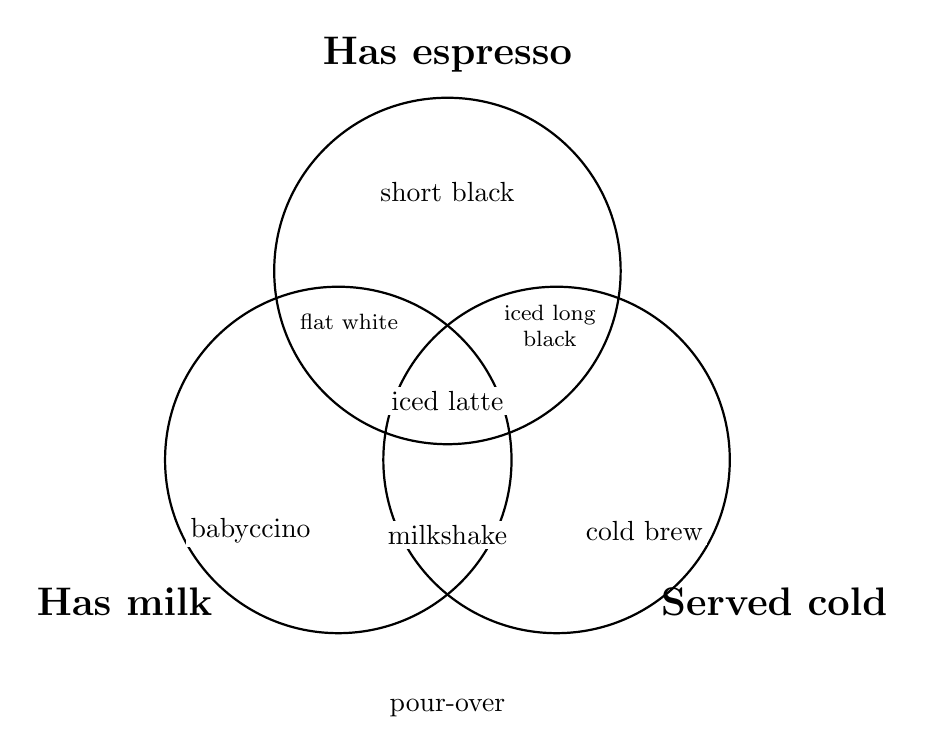
\begin{tikzpicture}
  \def\r{2.2}
  \coordinate (A) at (0,1.6);        % Has espresso
  \coordinate (B) at (-1.386,-0.8);  % Has milk
  \coordinate (C) at (1.386,-0.8);   % Served cold

  % Circles
  \draw[thick] (A) circle (\r);
  \draw[thick] (B) circle (\r);
  \draw[thick] (C) circle (\r);

  % Set labels
  \node[font=\Large\bfseries] at (0,4.35) {Has espresso};
  \node[font=\Large\bfseries] at (-4.1,-2.6) {Has milk};
  \node[font=\Large\bfseries] at (4.15,-2.6) {Served cold};

  % ---- Drinks in their regions ----
  % Espresso only
  \node[fill=white,inner sep=1.5pt] at (0,2.6) {short black};

  % Milk only
  \node[fill=white,inner sep=1.5pt] at (-2.5,-1.7) {babyccino};

  % Served cold only
  \node[fill=white,inner sep=1.5pt] at (2.5,-1.7) {cold brew};

  % Espresso + milk (not cold)
  \node[fill=white,inner sep=1pt,font=\footnotesize]
        at (-1.25,0.95) {flat white};

  % Espresso + cold (not milk)
  \node[fill=white,inner sep=1pt,font=\footnotesize,align=center]
        at (1.30,0.90) {iced long\\ black};

  % Milk + cold (not espresso)
  \node[fill=white,inner sep=1.5pt] at (0,-1.75) {milkshake};

  % All three
  \node[fill=white,inner sep=1.5pt] at (0,-0.05) {iced latte};

  % Outside all three sets
  \node[fill=white,inner sep=1.5pt] at (0,-3.95) {pour-over};
\end{tikzpicture}
\end{document}